% #----------------------------------------------#
% |   Autor Plantilla: Eduardo Cañete Carmona    |
% |   Fecha creación: 01/07/2019                 |
% |   Ultima actualización: 30/10/2026           |
% |   Versión: 3.13                              |
% #----------------------------------------------#



\documentclass[a4paper, 12pt]{book}
\usepackage[spanish,es-tabla]{babel}
\usepackage[utf8]{inputenc}

\usepackage[left = 35mm, right = 25mm, top = 25mm, height = 206mm]{geometry}
\usepackage{fancyhdr}
\usepackage{graphicx}
\usepackage{lipsum}
\usepackage[square,numbers]{natbib}
\usepackage[skip=12pt,font=small]{caption}  %Tamaño de la leyenda
\usepackage{subcaption}
\usepackage{amsmath}
\usepackage{afterpage}
\usepackage{titlesec}
\usepackage{color, colortbl}
\usepackage{listings}
\usepackage[dvipsnames,svgnames,table]{xcolor}
\usepackage{float}
\usepackage{eurosym}
\usepackage{enumitem}
\usepackage{amssymb}
\usepackage{array}
\usepackage{wrapfig}
\usepackage{multirow}
\usepackage{tabularx}
\usepackage{url}
\usepackage{eurosym}
\usepackage{appendix}
\usepackage{pdfpages}
\usepackage{pdflscape} %poner pdf horizontal
\usepackage[hidelinks]{hyperref}%para el hiperlink de las secciones
\usepackage[newfloat]{minted}
\usepackage[nottoc]{tocbibind}
\usepackage{glossaries}

\usepackage{booktabs}
\usepackage{pgfgantt}

\usepackage{diagbox}    % para la celda diagonal
\usepackage{colortbl}   % para \cellcolor y \rowcolor

\usepackage{soul}
\usepackage{xcolor}

\usepackage{ulem} %subrayado y tachado
\usepackage{pifont} % símbolos como tick y X
\usepackage{comment} % comentar bloques grandes
\usepackage{longtable} % diario de desarrollo (Anexo A)
\usepackage{seqsplit} % dividir texto largo automáticamente


\usepackage{tikz} % Diagramas de flujo
\usetikzlibrary{shapes.geometric, arrows} %Libería de flechas

% FONTs
\usepackage{fontenc}
\usepackage{textcomp}           % Needed for new symbols like € ?

%\usepackage[scaled]{berasans} % Font for the cover similar to Vera 33
%\renewcommand*\familydefault{\sfdefault}  %% To use as the base font of the document is to be sans serif

\usepackage{notoccite}

\usepackage{datetime}
%\newdateformat{monthyeardate}{\monthname, \THEYEAR}
\newcommand\Monthname[1][EMPTY]{
  \ifnum1=#1Enero\else
  \ifnum2=#1Febrero\else
  \ifnum3=#1Marzo\else
  \ifnum4=#1Abril\else
  \ifnum5=#1Mayo\else
  \ifnum6=#1Junio\else
  \ifnum7=#1Julio\else
  \ifnum8=#1Agosto\else
  \ifnum9=#1Septiembre\else
  \ifnum10=#1Octubre\else
  \ifnum11=#1Noviembre\else
  \ifnum12=#1Diciembre\else
  \fi\fi\fi\fi\fi\fi\fi\fi\fi\fi\fi\fi
}
\newdateformat{monthyeardate}{%
  \Monthname[\THEMONTH] \THEYEAR}
%\newdateformat{monthyeardate}{\Monthname[\THEMONTH], \THEYEAR}

% Entorno para código
\newenvironment{code}{\captionsetup{type=listing}}{}    

% Cambiamos el caption de los listing a español
\renewcommand{\listingname}{Código}    

 % Cambiamos el idioma del índice de códigos
\renewcommand*{\listlistingname}{Índice de Códigos}    

\newfloat{diagrama}{htbp}{loc}
\floatname{diagrama}{Diagrama}
\newcommand{\listofdiagrams}{\listof{diagrama}{Índice de Diagramas de Flujo}}
\floatstyle{plaintop}
\restylefloat{table}

\graphicspath{ {Imagenes/} }

\newcommand{\TipoTrabajo}{GRADO}
\newcommand{\TituloTFG}{Desarrollo de un dashboard inteligente para la gestión basada en datos: aplicación al rendimiento de corredores}
\newcommand{\TituloTFGIngles}{Development of an intelligent dashboard for data-driven management: application to runner performance}
\newcommand{\Grado}{Grado en Ingeniería Informática}
\newcommand{\AutorTFG}{Jorge Soriano Pijuan}
\newcommand{\DirectorUno}{D. Javier Pérez Barea}
\newcommand{\DirectorDos}{}
% Con un solo director, la portada pone "Director" (ver Portada/cover.tex).

% DNI: el repositorio es público, así que NO se escribe aquí.
% Crea el fichero local _datos_privados.tex (ignorado por git) con esta línea:
%   \newcommand{\DNI}{12345678X}
\IfFileExists{_datos_privados.tex}{\input{_datos_privados}}{\newcommand{\DNI}{\textit{[DNI]}}}

\definecolor{codegreen}{rgb}{0,0.6,0}
\definecolor{codegray}{rgb}{0.5,0.5,0.5}
\definecolor{codepurple}{rgb}{0.58,0,0.82}
\definecolor{backcolour}{rgb}{0.95,0.95,0.92}
% Colores corporativos de la EPSC (los mismos de la portada) para usar en el cuerpo
\definecolor{epscOscuro}{HTML}{280091}
\definecolor{epscMedio}{HTML}{4C5CC5}
\definecolor{epscVerde}{HTML}{00B299}

\lstdefinestyle{codestyle}{
    backgroundcolor=\color{backcolour},   
    commentstyle=\color{codegreen},
    keywordstyle=\color{magenta},
    numberstyle=\tiny\color{codegray},
    stringstyle=\color{codepurple},
    basicstyle=\ttfamily\footnotesize,
    breakatwhitespace=false,         
    breaklines=true,                 
    captionpos=b,                    
    keepspaces=true,                 
    %numbers=left,                    
    %numbersep=5pt,                  
    showspaces=false,                
    showstringspaces=false,
    showtabs=false,                  
    tabsize=2,
    literate=
    {á}{{\'a}}1 {é}{{\'e}}1 {í}{{\'i}}1 {ó}{{\'o}}1 {ú}{{\'u}}1
    {Á}{{\'A}}1 {É}{{\'E}}1 {Í}{{\'I}}1 {Ó}{{\'O}}1 {Ú}{{\'U}}1
    {à}{{\`a}}1 {è}{{\`e}}1 {ì}{{\`i}}1 {ò}{{\`o}}1 {ù}{{\`u}}1
    {À}{{\`A}}1 {È}{{\'E}}1 {Ì}{{\`I}}1 {Ò}{{\`O}}1 {Ù}{{\`U}}1
    {ä}{{\"a}}1 {ë}{{\"e}}1 {ï}{{\"i}}1 {ö}{{\"o}}1 {ü}{{\"u}}1
    {Ä}{{\"A}}1 {Ë}{{\"E}}1 {Ï}{{\"I}}1 {Ö}{{\"O}}1 {Ü}{{\"U}}1
    {â}{{\^a}}1 {ê}{{\^e}}1 {î}{{\^i}}1 {ô}{{\^o}}1 {û}{{\^u}}1
    {Â}{{\^A}}1 {Ê}{{\^E}}1 {Î}{{\^I}}1 {Ô}{{\^O}}1 {Û}{{\^U}}1
    {œ}{{\oe}}1 {Œ}{{\OE}}1 {æ}{{\ae}}1 {Æ}{{\AE}}1 {ß}{{\ss}}1
    {ç}{{\c c}}1 {Ç}{{\c C}}1 {ø}{{\o}}1 {å}{{\r a}}1 {Å}{{\r A}}1
    {€}{{\EUR}}1 {£}{{\pounds}}1 {ñ}{{\~{n}}}1
}
\tikzstyle{startstop} = [rectangle, rounded corners, 
minimum width=3cm, 
minimum height=1cm,
text centered, 
draw=black, 
fill=red!30]

\tikzstyle{io} = [trapezium, 
trapezium stretches=true, % A later addition
trapezium left angle=70, 
trapezium right angle=110, 
minimum width=3cm, 
minimum height=1cm, text centered, 
draw=black, fill=blue!30]

\tikzstyle{process} = [rectangle, 
minimum width=3cm, 
minimum height=1cm, 
text centered, 
text width=3cm, 
draw=black, 
fill=orange!30]

\tikzstyle{decision} = [diamond, 
minimum width=3cm, 
minimum height=1cm, 
text centered, 
draw=black, 
fill=green!30]
\tikzstyle{arrow} = [thick,->,>=stealth]
%----------------------------------------------------------------------------------------
%	ENCABEZADOS Y PIE DE PAGINA
%----------------------------------------------------------------------------------------

\pagestyle{fancy}
	\fancypagestyle{cuerpo}{
      \fancyfoot{}
      \fancyfoot[L]{Trabajo Fin de Grado} %Autor
      \fancyfoot[C]{}
      \fancyfoot[R]{- \thepage \ -}
      \fancyhead{}
      \fancyhead[L]{\leftmark} %Nombre del documento
      \fancyhead[R]{
\includegraphics[height=1.8cm]{Portada/Img/logoUCO.pdf}} %Logo Universidad
      \renewcommand{\headrulewidth}{0.4pt}
      \renewcommand{\footrulewidth}{0.4pt}
      \setlength{\headheight}{65pt}
    }
    \fancypagestyle{indice}{
      \fancyfoot{}
      \fancyfoot[L]{\AutorTFG} %Autor
      \fancyfoot[R]{- \thepage \ -} %Asignatura
      \fancyhead{}
      \fancyhead[L]{Trabajo Fin de Grado} %Nombre del documento
      \fancyhead[R]{
\includegraphics[height=1.8cm]{Portada/Img/logoUCO.pdf}} %Logo
      \renewcommand{\headrulewidth}{0.4pt}
      \renewcommand{\footrulewidth}{0.4pt}
      \setlength{\headheight}{65pt}
      }
      
    \fancypagestyle{plain}{% % <-- this is new
     \fancyfoot{}
      \fancyfoot[L]{Trabajo Fin de Grado} %Autor
      \fancyfoot[C]{} %ecc
      \fancyfoot[R]{- \thepage \ -}
      \fancyhead{}
      \fancyhead[L]{\leftmark} %Nombre del documento
      \fancyhead[R]{
\includegraphics[height=1.8cm]{Portada/Img/logoUCO.pdf}} %Logo Universidad
      \renewcommand{\headrulewidth}{0.4pt}
      \renewcommand{\footrulewidth}{0.4pt}
      \setlength{\headheight}{65pt}
    }
  
\setcounter{secnumdepth}{4}

\pagenumbering{empty}


%%%%%%%%%
% ANEXO %
%%%%%%%%%

% Para que ponga ANEXO en vez de APENDICE
 \addto\captionsspanish{\renewcommand{\appendixname}{Anexo}} %para que ponga anexo y no apéndice.

\makeglossaries
\raggedbottom  % Quita huecos grandes en blanco
\begin{document}

%%%%%%%%%%%
% PORTADA %
%%%%%%%%%%%
\begingroup  % <- inicio del grupo

\fontfamily{fvs}\selectfont  % Bera Sans solo aquí
% Definición de colores usados en la portada
\definecolor{epsc:oscuro}{HTML}{280091}
\definecolor{epsc:medio}{HTML}{4C5CC5}
\definecolor{epsc:verde}{HTML}{00B299}
\definecolor{epsc:claro}{HTML}{3FCFD5}

\definecolor{friendlyGray}{HTML}{f0f0f0}

\thispagestyle{empty}
\null
\vspace*{2.5cm}

\begin{tikzpicture}[remember picture, overlay]
  % Top
  \node [anchor=north east, inner sep=0pt]  at (current page.north east)%
    {
\includegraphics[height=6cm]{Portada/Img/topRightCorner.pdf}};
  % Bottom
  \node [anchor=south west, inner sep=0pt]  at (current page.south west)%
    {
\includegraphics[height=6cm]{Portada/Img/bottomLeftCorner.pdf}};
  \node (uco) [anchor=south east, inner sep=0pt, xshift=-10mm, yshift=10mm]  at (current page.south east)%
    {
\includegraphics[height=2cm]{Portada/Img/logoUCO.pdf}};
  \node [anchor=south east, inner sep=0pt, xshift=-10mm]  at (uco.south west)%
    %{
\includegraphics[height=2cm]{Portada/Img/emblema-vacio.png}};
    %{
\includegraphics[height=2cm]{Portada/Img/emblema-ing-tec-industrial.png}};
    {
\includegraphics[height=2cm]{Portada/Img/emblema-ing-informatica.pdf}};
    %{
\includegraphics[height=2cm]{Portada/Img/emblema-master-ing-industrial.pdf}};
\end{tikzpicture}

\begin{center}

\includegraphics[width=12.5cm]{Portada/Img/LogotipoEPSC.pdf}
\end{center}

\vfill

\begin{center}
\large\textbf{\color{epsc:medio}
\fontencoding{T1}\selectfont
  TRABAJO FIN DE \TipoTrabajo
}
\end{center}

\vfill

\begin{center}
\Large\textbf{\color{epsc:verde}
\fontencoding{T1}\selectfont
  \Grado
}
\end{center}

\vspace{0.5cm}

\begin{center}
\Huge\textbf{\color{epsc:oscuro} % Huge / huge / LARGE / Large / large / normalsize
\fontencoding{T1}\selectfont
  \TituloTFG
}
\end{center}

\begin{center}
\normalsize{\color{epsc:medio}
\fontencoding{T1}\selectfont
  \TituloTFGIngles
}
\end{center}

\vfill

{
\begin{center}
\fontencoding{T1}\selectfont
\large{\color{epsc:oscuro}Autor}\\
\textbf{\color{epsc:medio} \AutorTFG }
\end{center}
}


\vfill

{
\begin{center}
\fontencoding{T1}\selectfont
\large{\color{epsc:oscuro} Director }\\
\textbf{\color{epsc:medio} \DirectorUno }
\end{center}
}

\vfill

{
\begin{center}
\fontencoding{T1}\selectfont
\textbf{\color{epsc:verde} \monthyeardate\today}
\end{center}
}

\endgroup  % <- fin del grupo, la fuente vuelve a la normal

\endinput

\newpage
\thispagestyle{empty}   % Página en blanco entre la portada y el comienzo del documento
\mbox{} 
$\ $
\thispagestyle{empty} % para que no se numere esta pagina
%\newpage
%$\ $
%\thispagestyle{empty} % para que no se numere esta pagina

%%%%%%%%%%%%%%%%%%%%%%%%%%
% ANEXO V - Originalidad %
%%%%%%%%%%%%%%%%%%%%%%%%%%
%--------------------------------------
% ANEXO V - Declaración de originalidad 
%--------------------------------------
%\newcommand{\TipoTrabajo}{GRADO}
\newcommand{\TituloTFG}{Desarrollo de un dashboard inteligente para la gestión basada en datos: aplicación al rendimiento de corredores}
\newcommand{\TituloTFGIngles}{Development of an intelligent dashboard for data-driven management: application to runner performance}
\newcommand{\Grado}{Grado en Ingeniería Informática}
\newcommand{\AutorTFG}{Jorge Soriano Pijuan}
\newcommand{\DirectorUno}{D. Javier Pérez Barea}
\newcommand{\DirectorDos}{}
% Con un solo director, la portada pone "Director" (ver Portada/cover.tex).

% DNI: el repositorio es público, así que NO se escribe aquí.
% Crea el fichero local _datos_privados.tex (ignorado por git) con esta línea:
%   \newcommand{\DNI}{12345678X}
\IfFileExists{_datos_privados.tex}{\input{_datos_privados}}{\newcommand{\DNI}{\textit{[DNI]}}}


\definecolor{griscampo}{gray}{0.9}

\newgeometry{left=2cm,right=2cm,top=2.5cm,bottom=2.5cm}

\thispagestyle{empty}

\begin{table}[h]
\centering
\begin{tabular}{|m{3cm}|m{9cm}|m{3cm}|}
\hline
\centering

\includegraphics[width=2.5cm,height=2.5cm]{AnexoV/Img/logo_uco_final.png}
&
\centering
\textbf{ANEXO V}\\
Escuela Politécnica Superior de Córdoba\\
\textbf{DECLARACIÓN DE ORIGINALIDAD DEL TFG}
&
\centering

\includegraphics[width=2.5cm,height=2.5cm]{AnexoV/Img/logo_epsc_final.png}
\tabularnewline
\hline
\end{tabular}
\end{table}

\vspace{0.8cm}

\noindent D./D.ª \colorbox{griscampo}{\AutorTFG}, con DNI \colorbox{griscampo}{\DNI}

\vspace{0.5cm}

\noindent Estudiante del \colorbox{griscampo}{\Grado}

\vspace{0.9cm}

\noindent \textbf{D E C L A R A:}\\
\noindent Que es el/la autor/a y asume la originalidad, entendida esta última en el sentido de que no ha utilizado fuentes sin citarlas debidamente, del Trabajo Fin de Grado titulado:\\
\colorbox{griscampo}{\parbox{\linewidth}{\TituloTFG}}

\vspace{1.5 cm}

\noindent Asimismo, es consciente de que el plagio, entendido como la presentación de un trabajo u obra hecho por otra persona como propio o la copia de textos sin citar su procedencia, conllevará automáticamente la calificación numérica de cero y que esta consecuencia se entiende sin perjuicio de las responsabilidades disciplinarias en las que pudieran incurrir si plagia, al tener la consideración de infracción muy grave, de conformidad con el artículo 11.g de la Ley 3/2022, de Convivencia Universitaria y artículo 8.g del Reglamento 5/2023 de Convivencia Universitaria de la Universidad de Córdoba.

\vspace{0.9cm}

\noindent En Córdoba, a \today

\vspace{1.0cm}

\begin{center}
\noindent El/la estudiante
\end{center}

\vspace{2cm}

\begin{center}   
\noindent Fdo.: \AutorTFG%\underline{\hspace{8cm}}

%\vspace{4cm}
\vfill
Sr. Director de la Escuela Politécnica Superior de Córdoba.

\end{center}

\restoregeometry

\endinput



%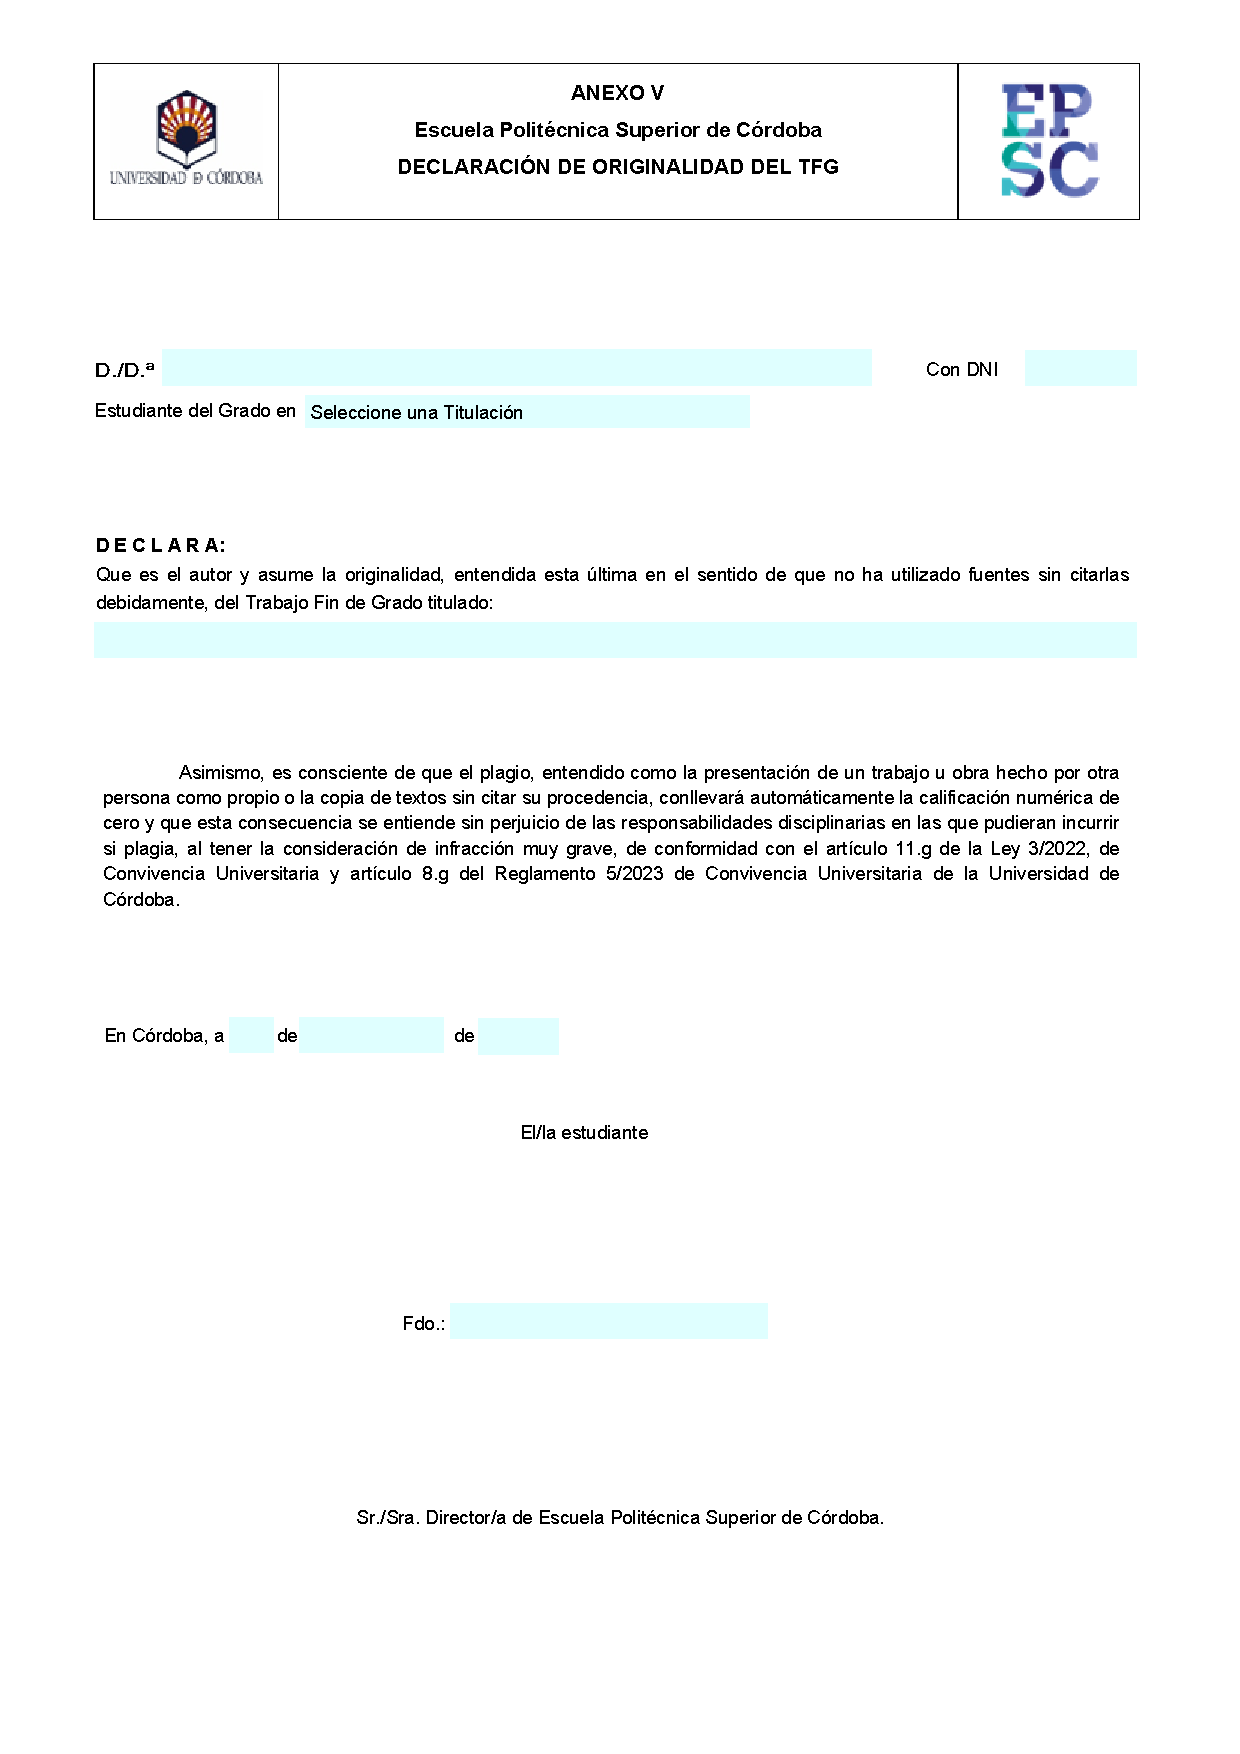
\includepdf[pages=-]{AnexoV/AnexoV_DECLARACION_ORIGINALIDAD_TFG.PDF}
\newpage
\thispagestyle{empty}
\mbox{}
\newpage

%%%%%%%%%%%%%%%
% DEDICATORIA %
%%%%%%%%%%%%%%%
\pagenumbering{Roman} % para comenzar la numeracion de paginas en numeros romanos
\pagestyle{indice}
\thispagestyle{indice}
% REVISAR: dedicatoria personal
\begin{flushright}
\textit{Dedicado a \\
mi familia}
\end{flushright}

%%%%%%%%%%%%%%%%%%%
% AGRADECIMIENTOS %
%%%%%%%%%%%%%%%%%%%
\chapter*{Agradecimientos}

\addcontentsline{toc}{chapter}{Agradecimientos} % si queremos que aparezca en el índice

\markboth{Agradecimientos}{Agradecimientos} % encabezado

% TODO: redactar al final del proyecto.


%%%%%%%%%%%%%%%%%%%%%%
% RESUMEN Y ABSTRACT %
%%%%%%%%%%%%%%%%%%%%%%
% Obligatorio (Reglamento 24/2024 TFG EPSC, art. 9.1): resumen y palabras clave en español
% y en inglés. Se redacta al final, cuando haya resultados.

\chapter*{Resumen}
\addcontentsline{toc}{chapter}{Resumen} % si queremos que aparezca en el índice
\markboth{Resumen}{Resumen} % encabezado

% TODO: resumen (motivación, qué se ha hecho, resultados principales).

% REVISAR: palabras clave provisionales.
\textbf{Palabras clave:} \textit{dashboard}, análisis de datos, rendimiento deportivo, carrera a pie, series temporales.

\chapter*{Abstract}
\addcontentsline{toc}{chapter}{Abstract} % si queremos que aparezca en el índice
\markboth{Abstract}{Abstract} % encabezado

% TODO: English version of the summary.

\textbf{Keywords:} dashboard, data analytics, sports performance, running, time series.


%%%%%%%%%%%%%%%%%%
% INDICE GENERAL %
%%%%%%%%%%%%%%%%%%
\newpage
\thispagestyle{fancy} 

\tableofcontents

\cleardoublepage
\listoffigures

\cleardoublepage
\listoftables

% Índice de diagramas de flujo: descomentar cuando se use el entorno «diagrama».
%\cleardoublepage
%\phantomsection
%\addcontentsline{toc}{chapter}{Índice de diagramas de flujo}
%\listofdiagrams

\cleardoublepage
\phantomsection
\addcontentsline{toc}{chapter}{Lista de Acrónimos}

% Acrónimos. Solo aparecen en la lista los que se usan en el texto con \gls{clave}.
% Primera aparición: forma larga + (corta); siguientes: forma corta.

\newacronym{api}{API}{Application Programming Interface}
\newacronym{adr}{ADR}{Architecture Decision Record}
\newacronym{acwr}{ACWR}{Acute:Chronic Workload Ratio}
\newacronym{fc}{FC}{frecuencia cardíaca}
\newacronym{fit}{FIT}{Flexible and Interoperable Data Transfer}
\newacronym{gps}{GPS}{Global Positioning System}
\newacronym{gpx}{GPX}{GPS Exchange Format}
\newacronym{ia}{IA}{inteligencia artificial}
\newacronym{xml}{XML}{Extensible Markup Language}
\newacronym{mae}{MAE}{Mean Absolute Error}
\newacronym{rmse}{RMSE}{Root Mean Square Error}
\newacronym{tfg}{TFG}{Trabajo Fin de Grado}
\newacronym{trimp}{TRIMP}{Training Impulse}

\printglossary[type=\acronymtype, title={Acrónimos}]

%---------------------%
%	CUERPO DE TEXTO   %
%---------------------%

\afterpage{\null\newpage}

\newpage
\newpage

\pagestyle{cuerpo}
\thispagestyle{cuerpo}

\pagenumbering{arabic}

%%%%%%%%%%%%%%%%%%%%%%%%%%%%%%%%%%%%%%%%%%%%%%%%%%%%%%%%%%%%%%%%%%%%%
%                         ESTRUCTURA CONTENIDO                      %
%%%%%%%%%%%%%%%%%%%%%%%%%%%%%%%%%%%%%%%%%%%%%%%%%%%%%%%%%%%%%%%%%%%%%

%------------------%
%	CAPÍTULOS      %
%------------------%

% Estructura según la propuesta aprobada (ver 4_metodologia.tex, partes 1--5)
\chapter{Introducción}
\label{ch:introduccion}

% TODO: redactar la introducción (contexto, motivación y estructura de la memoria).
% Los ejemplos de LaTeX de la plantilla están en EJEMPLOS_LATEX.tex.


En estas primeras líneas de texto se puede ver como se cita una referencia bibliográfica contenida en el archivo ``referencias.bib''. En \cite{ref_articulo} se hace referencia a un artículo, en \cite{ref_libro} se hace referencia a un libro y en \cite{ref_web} se hace referencia a una web. 


\chapter{Objetivos}
\label{ch:objetivos}

% Los objetivos deben coincidir con los de la propuesta aprobada (anteproyecto).
% No modificar su contenido sin acordarlo con el tutor.

\section{Objetivo general}
\label{sec:objetivo_general}

El objetivo general de este trabajo es desarrollar un \textit{dashboard} inteligente que integre datos de rendimiento de corredores, detecte patrones de evolución y estime la progresión del rendimiento, como herramienta de apoyo a la toma de decisiones basada en datos.

\section{Objetivos específicos}
\label{sec:objetivos_especificos}

Para alcanzar el objetivo general se plantean los siguientes objetivos específicos, recogidos en la propuesta aprobada:

\begin{enumerate}[label=\textbf{O\arabic*.}, leftmargin=*]
    \item \label{obj:dashboard} Diseñar e implementar un \textit{dashboard} interactivo que integre datos de rendimiento obtenidos de plataformas y dispositivos deportivos (como Strava o Garmin), permitiendo la visualización dinámica de métricas individuales y grupales.
    \item \label{obj:analisis} Desarrollar un modelo de análisis de datos deportivos que permita detectar patrones de evolución en el ritmo, la frecuencia cardíaca, la potencia y la distancia recorrida, utilizando técnicas estadísticas y de ingeniería de datos.
    \item \label{obj:prediccion} Implementar un módulo predictivo basado en regresión lineal y modelos de series temporales para estimar la progresión del rendimiento del corredor a corto y medio plazo.
    \item \label{obj:interfaz} Diseñar una interfaz visual optimizada, intuitiva y adaptable, que facilite la interpretación de los indicadores de rendimiento tanto para deportistas individuales como para entrenadores o equipos.
    \item \label{obj:datos} Integrar un sistema de gestión de datos estructurados que permita la comparación de resultados entre distintos corredores, fomentando la toma de decisiones basada en evidencias y el seguimiento personalizado del progreso.
\end{enumerate}

La Tabla \ref{tab:objetivos_capitulos} relaciona cada objetivo con el capítulo de la memoria en el que se aborda.

\begin{table}[H]
\centering
\caption{Relación entre objetivos específicos y capítulos de la memoria.}
\label{tab:objetivos_capitulos}
\begin{tabular}{@{}cll@{}}
\toprule
\textbf{Objetivo} & \textbf{Ámbito} & \textbf{Capítulo} \\
\midrule
O1 & \textit{Dashboard} interactivo & \ref{ch:dashboard} \\
O2 & Análisis de patrones & \ref{ch:predictivo} \\
O3 & Módulo predictivo & \ref{ch:predictivo} \\
O4 & Interfaz y usabilidad & \ref{ch:dashboard} y \ref{ch:evaluacion} \\
O5 & Gestión de datos estructurados & \ref{ch:modelo_datos} \\
\bottomrule
\end{tabular}
\end{table}

\chapter{Antecedentes}
\label{ch:antecedentes}

% Fuente: apartado «Antecedentes» de la propuesta aprobada.
% TODO: desarrollar cada sección con fuentes verificadas (ver TODO en referencias.bib).

El auge de los dispositivos \textit{wearables} (Garmin, Polar, Suunto) y de plataformas como Strava o TrainingPeaks ha impulsado la generación masiva de datos de rendimiento deportivo. Sin embargo, la mayoría de estos sistemas presentan interfaces cerradas o de uso limitado para análisis personalizados. El desarrollo de \textit{dashboards} propios mediante herramientas como Power BI, Python (Dash, Streamlit) o React permite crear soluciones adaptadas a las necesidades del usuario final, integrando múltiples fuentes y técnicas de análisis predictivo.

Este trabajo se enmarca dentro de las metodologías de gestión basada en datos (\textit{Data-Driven Management}) aplicadas al contexto deportivo \cite{davenport2010analytics, marr2016big}.

\section{Dispositivos y plataformas de registro deportivo}
\label{sec:plataformas}
% TODO: relojes GPS y sensores (FC, potencia, cadencia); plataformas (Strava, Garmin Connect,
% TrainingPeaks); qué análisis ofrecen y sus limitaciones (interfaces cerradas, exportación).

\section{Métricas de rendimiento en carrera}
\label{sec:metricas}
% TODO: ritmo y velocidad, \gls{fc} y zonas, cadencia, potencia.
% TODO: carga de entrenamiento (\gls{trimp}), relación carga aguda/crónica (\gls{acwr}),
% eficiencia aeróbica, predicción de marcas (fórmula de Riegel). Cada una con su fuente.

\section{Técnicas de análisis y predicción}
\label{sec:tecnicas}
% TODO: regresión lineal y series temporales \cite{montgomery2018applied}; aprendizaje
% automático aplicado \cite{geron2022hands}; validación temporal de modelos.

\section{Herramientas para el desarrollo de \textit{dashboards}}
\label{sec:herramientas_dashboard}
% TODO: comparativa Power BI, Streamlit, Dash, React (criterios: control de la interfaz,
% integración de modelos propios, versionado, coste). Enlaza con la decisión del ADR 0001.

\section{Conclusiones del estudio de antecedentes}
\label{sec:conclusiones_antecedentes}
% TODO: qué hueco cubre este trabajo frente a las soluciones existentes.

\chapter{Metodología, planificación y recursos}
\label{ch:metodologia}

% Fuente: apartados «Partes del TFG», «Fases de desarrollo y cronograma» y «Recursos previstos»
% de la propuesta aprobada.

\section{Metodología de trabajo}
\label{sec:metodologia}

El desarrollo sigue un enfoque incremental: cada fase produce un resultado funcional que se revisa con el tutor antes de iniciar la siguiente. Siguiendo sus indicaciones, el alcance y las funcionalidades se ajustan en función del tiempo disponible y de los avances conseguidos, para que el trabajo resulte viable y permita profundizar adecuadamente en los resultados.

El trabajo se organiza en cinco partes, que se corresponden con los capítulos \ref{ch:analisis_datos} a \ref{ch:evaluacion}:

\begin{enumerate}
    \item \textbf{Análisis del contexto y recopilación de datos:} estudio del entorno deportivo, identificación de fuentes relevantes (\gls{api} de Strava o Garmin Connect, sensores o \textit{datasets} simulados) y definición de las métricas de rendimiento más representativas.
    \item \textbf{Diseño del modelo de datos:} estructuración de la información mediante un esquema relacional o modelo de entidades y relaciones, garantizando la coherencia, trazabilidad y escalabilidad del sistema.
    \item \textbf{Desarrollo del \textit{dashboard} inteligente:} implementación del panel interactivo con gráficos dinámicos, filtros personalizados y visualización simultánea de datos individuales y grupales.
    \item \textbf{Módulo analítico y predictivo:} funciones estadísticas y modelos de predicción basados en regresión y series temporales para estimar la evolución del rendimiento y generar alertas de mejora o desviación.
    \item \textbf{Evaluación y validación del sistema:} pruebas funcionales del \textit{dashboard}, análisis de la precisión de los modelos predictivos y validación del diseño desde el punto de vista técnico y de usabilidad.
\end{enumerate}

Las decisiones técnicas relevantes se documentan como registros de decisiones de arquitectura (\gls{adr}) en el repositorio del proyecto, y cada sesión de trabajo se anota en el diario de desarrollo (Anexo \ref{anx:diario}).

\section{Planificación}
\label{sec:planificacion}

La Figura \ref{fig:cronograma} muestra el cronograma previsto en la propuesta, con una duración de doce semanas.

\begin{figure}[H]
\centering
\begin{ganttchart}[
    hgrid, vgrid,
    x unit=0.7cm, y unit chart=0.75cm,
    title height=1,
    bar/.append style={fill=epscMedio!70},
    bar label font=\small,
    title label font=\small
  ]{1}{12}
  \gantttitle{Semana}{12} \\
  \gantttitlelist{1,...,12}{1} \\
  \ganttbar{F1. Requisitos, datos y modelo}{1}{3} \\
  \ganttbar{F2. \textit{Dashboard} e integración}{4}{6} \\
  \ganttbar{F3. Módulo analítico y predictivo}{7}{8} \\
  \ganttbar{F4. Validación y documentación}{9}{10} \\
  \ganttbar{F5. Memoria final y defensa}{11}{12}
\end{ganttchart}
\caption{Cronograma previsto del proyecto.}
\label{fig:cronograma}
\end{figure}

% TODO: al cierre de cada fase, comparar lo previsto con lo real (desviaciones y causas).

\section{Recursos}
\label{sec:recursos}

\begin{table}[H]
\centering
\caption{Recursos empleados en el proyecto.}
\label{tab:recursos}
\begin{tabularx}{\textwidth}{@{}lX@{}}
\toprule
\textbf{Tipo} & \textbf{Recursos} \\
\midrule
Lenguaje y librerías & Python: pandas, Plotly, Dash, scikit-learn, statsmodels, SQLAlchemy, fitparse, gpxpy \\
Persistencia & SQLite \\
Fuentes de datos & Exportaciones de Strava y Garmin Connect (formatos \gls{fit} y \gls{gpx}) o \textit{datasets} simulados \\
Control de versiones & Git y GitHub \\
Entorno de desarrollo & Visual Studio Code, Jupyter Notebook \\
Documentación & \LaTeX{} (plantilla de TFG de la EPSC) \\
Infraestructura & Ordenador personal con entorno de desarrollo local \\
\bottomrule
\end{tabularx}
\end{table}

% REVISAR: la propuesta preveía también JavaScript (React, Chart.js) y Power BI / Streamlit como
% alternativas. Se eligió Dash para todo el sistema (ver ADR 0001 y sección \ref{sec:herramientas_dashboard}).

\subsection{Uso de herramientas de inteligencia artificial}
\label{sec:uso_ia}

Durante el desarrollo se han utilizado asistentes de \gls{ia} (Claude Code y opencode) como apoyo en la programación, la configuración del entorno y la revisión de la documentación. Las convenciones que siguen estas herramientas están documentadas en el repositorio del proyecto. Todas las decisiones de diseño, el código y el contenido de esta memoria han sido revisados y asumidos por el autor.
% REVISAR: confirmar con el tutor el nivel de detalle requerido sobre el uso de IA.

\chapter{Análisis del contexto y recopilación de datos}
\label{ch:analisis_datos}

% Parte 1 de la propuesta (Fase 1, semanas 1--3).
% Estudio del entorno deportivo, identificación de fuentes relevantes (APIs como Strava o Garmin
% Connect, sensores o datasets simulados) y definición de las métricas más representativas.

\section{Fuentes de datos}
\label{sec:fuentes}

Los datos de entrenamiento reales de este trabajo proceden de la aplicación adidas Running (antes Runtastic), que es la única plataforma en la que el autor ha registrado sus sesiones. La sincronización automática con esta plataforma no es posible, ya que adidas retiró su \gls{api} pública el 30 de junio de 2025 \cite{runalyze2025changelog}. Por tanto, los datos se obtienen mediante la exportación manual de la cuenta, que entrega un fichero comprimido con un documento \gls{json} por sesión y las series de posición y, cuando se registró, de \gls{fc}.

Se ha optado por leer esta exportación en su formato original, en lugar de convertirla antes a formatos más extendidos como \gls{fit} o \gls{gpx}. La justificación de esta decisión y su efecto en la arquitectura del sistema se describen en la sección~\ref{sec:ingesta}.

% TODO: tras explorar la exportación real, detallar los campos disponibles en cada sesión y sus
% limitaciones (en especial, si hay frecuencia cardiaca, necesaria para el TRIMP).
% TODO: fuente de los datos de varios corredores para la vista de entrenador (pendiente de decidir).

\section{Formatos de las actividades}
\label{sec:formatos}
% TODO: \gls{fit}, \gls{gpx} (y TCX si aparece). Campos disponibles, frecuencia de muestreo,
% unidades y conversiones (p. ej. cadencia por pierna, coordenadas en semicírculos).

\section{Exploración de los datos}
\label{sec:exploracion}
% TODO: resultados del notebook de exploración: cobertura de cada campo, calidad de los datos
% (pausas, saltos de \gls{gps}, valores fuera de rango).

\section{Métricas de rendimiento seleccionadas}
\label{sec:metricas_seleccionadas}
% TODO: métricas que se calcularán y por qué (enlaza con la sección \ref{sec:metricas}).

\section{Requisitos del sistema}
\label{sec:requisitos}
% TODO: requisitos funcionales y no funcionales, con identificador (RF-01, RNF-01...) y
% trazabilidad con los objetivos O1--O5.
       % Parte 1
\chapter{Diseño del modelo de datos}
\label{ch:modelo_datos}

% Parte 2 de la propuesta (Fase 1, semanas 1--3). Cubre el objetivo O5.
% Estructuración de la información mediante un esquema relacional o modelo entidad-relación,
% garantizando coherencia, trazabilidad y escalabilidad.

\section{Arquitectura general del sistema}
\label{sec:arquitectura}
% TODO: diagrama de componentes (ingesta, almacenamiento, análisis, dashboard).

\section{Modelo conceptual}
\label{sec:modelo_conceptual}
% TODO: entidades (corredor, actividad, muestra, métricas...) y relaciones. Diagrama E-R.

\section{Esquema relacional}
\label{sec:esquema_relacional}
% TODO: tablas, claves y restricciones; implementación con SQLite y SQLAlchemy.

\section{Proceso de ingesta y transformación}
\label{sec:ingesta}

La ingesta se ha diseñado para que el resto del sistema no dependa del formato en que se exportan los datos. Para ello se aplica el patrón adaptador: cada fuente de datos dispone de un adaptador propio que lee los ficheros de esa fuente y los transforma en un esquema canónico común, con unidades del Sistema Internacional, marcas de tiempo en UTC y nombres de columna fijos. El adaptador es el único componente que conoce el formato de origen, de modo que las conversiones de unidades y de campos se realizan una sola vez y en un único lugar. El modelo de datos, el cálculo de métricas y el \textit{dashboard} trabajan exclusivamente con el esquema canónico.

El primer adaptador lee la exportación de la aplicación Salud de Apple (sección~\ref{sec:fuentes}). El documento \gls{xml} principal ocupa cerca de 1~GB, por lo que se recorre en modo secuencial con la biblioteca estándar de Python, sin cargarlo entero en memoria; las rutas \gls{gpx} se leen con la biblioteca gpxpy. El adaptador conserva únicamente las carreras registradas por el Apple Watch y descarta las escritas por otras aplicaciones. De este modo, todas las sesiones se miden con el mismo sensor y los mismos algoritmos, y no es necesaria una regla de eliminación de duplicados.

Se descartaron las siguientes alternativas:

\begin{itemize}
    \item Usar la exportación de la cuenta de adidas Running, porque solo cubre las sesiones de esa aplicación y no incluye rutas ni métricas de dinámica de carrera.
    \item Combinar todos los orígenes de la exportación con una regla de eliminación de duplicados. Aportaría más sesiones, pero mezclaría sensores y algoritmos de cálculo distintos, de modo que las métricas dejarían de ser comparables entre sesiones.
    \item Convertir los datos a \gls{fit} con un servicio externo, porque añade un paso manual y una dependencia ajena al proyecto, y la conversión puede alterar campos sin que quede constancia en el código.
    \item Leer el formato de origen directamente desde el modelo y las métricas, sin capa de adaptación, porque acoplaría todo el sistema a un formato concreto.
\end{itemize}

Esta elección tiene un coste conocido: se descartan las sesiones registradas solo con otras aplicaciones y, en los entrenamientos del reloj, la \gls{fc} por muestra aparece agregada en la exportación. Por ello, la carga de entrenamiento se calculará con métricas basadas en la \gls{fc} media de la sesión.

La principal consecuencia de esta decisión es la extensibilidad: incorporar otra fuente de datos, como un reloj que exporte ficheros \gls{fit}, solo requiere escribir un nuevo adaptador con sus pruebas, sin modificar el modelo de datos ni el resto del flujo. La decisión se documenta en el ADR 0004 del repositorio.

% TODO: diagrama del flujo (exportación, adaptador, esquema canónico, SQLite) y reglas de limpieza
% aplicadas (pausas, saltos de GPS, FC fuera de rango) cuando estén implementadas.
  % Parte 2
\chapter{Desarrollo del \textit{dashboard}}
\label{ch:dashboard}

% Parte 3 de la propuesta (Fase 2, semanas 4--6). Cubre los objetivos O1 y O4.
% Panel interactivo con gráficos dinámicos, filtros personalizados y visualización simultánea de
% datos individuales y grupales.

\section{Diseño de la interfaz}
\label{sec:diseno_interfaz}
% TODO: público objetivo (corredor, entrenador), vistas y bocetos.

\section{Implementación}
\label{sec:implementacion_dashboard}
% TODO: estructura de la aplicación Dash, componentes, callbacks y conexión con los datos.

\section{Visualizaciones}
\label{sec:visualizaciones}
% TODO: gráficos de cada vista y qué decisión ayudan a tomar.

\section{Vista individual y vista grupal}
\label{sec:vistas}
% TODO: seguimiento de un corredor y comparación entre corredores.
            % Parte 3
\chapter{Módulo analítico y predictivo}
\label{ch:predictivo}

% Parte 4 de la propuesta (Fase 3, semanas 7--8). Cubre los objetivos O2 y O3.
% Funciones estadísticas y modelos de predicción basados en regresión y series temporales para
% estimar la evolución del rendimiento y generar alertas de mejora o desviación.

\section{Análisis de patrones de evolución}
\label{sec:patrones}
% TODO: evolución de ritmo, \gls{fc}, potencia y distancia; métricas de carga y eficiencia.

\section{Modelos predictivos}
\label{sec:modelos}
% TODO: regresión lineal y series temporales \cite{montgomery2018applied, geron2022hands}.
% Variables de entrada, horizonte de predicción (corto y medio plazo).

\section{Metodología de evaluación de los modelos}
\label{sec:evaluacion_modelos}
% TODO: división temporal de los datos, modelo de referencia (línea base), métricas
% \gls{mae} y \gls{rmse}.

\section{Alertas de mejora o desviación}
\label{sec:alertas}
% TODO: reglas o umbrales y cómo se muestran en el dashboard.
    % Parte 4
\chapter{Evaluación y validación}
\label{ch:evaluacion}

% Parte 5 de la propuesta (Fase 4, semanas 9--10).
% Pruebas funcionales del dashboard, análisis de precisión de los modelos predictivos y
% validación del diseño desde el punto de vista técnico y de usabilidad.

\section{Pruebas funcionales}
\label{sec:pruebas_funcionales}
% TODO: estrategia de pruebas (pytest), cobertura y resultados.

\section{Precisión de los modelos predictivos}
\label{sec:precision}
% TODO: resultados frente a la línea base, con sus limitaciones.

\section{Validación de usabilidad}
\label{sec:usabilidad}
% TODO: prueba con usuarios (corredores / entrenador), método y resultados.

\section{Discusión de resultados}
\label{sec:discusion}
% TODO: interpretación de los resultados obtenidos.
           % Parte 5

% Ejemplos de la plantilla: descomentar solo para consultarlos (no van en la memoria)
%\chapter{Ejemplos de código Latex}
\label{ch:codigos_ejemplo}
Aquí también se puede poner texto.

\section{Acrónimos}
Ejemplo de como poner un acrónimo \acrshort{iot}. Estos están definidos en el archivo ``anexo\_acronimos.text''.


\section{Comillas}
Mira el código para que veas como se hace bien el ``entrecomillado''. No se usan las comillas situadas en la tecla del dígito 2.

\subsection{seccion prueba}
asdf

\subsubsection{seccion prueba}
asdf

\section{Listas}
En esta sección se muestra como crear dos tipos de listas.

\subsection{Lista Enumerada}
\begin{enumerate}
\item Color rojo
\item Color verde
\item Color amarillo
\end{enumerate}



\subsection{Lista NO-Enumerada}
\begin{itemize}
\item Color rojo
\item Color verde
\item Color amarillo
\end{itemize}

\section{Como incluir FIGURAS}

\subsection{Figura única}
\label{sec:figura_unica}

\begin{figure}[H]
  \centering
  % include first image
  
\includegraphics[width=.8\linewidth]{Imagenes/ejemplo.png}  
  \caption[Titulo de la figura para el índice de figuras. En este no se deben poner referencias a citas]{Título de la figura para el texto}
  \label{fig:figura_unica}
\end{figure}

\subsection{Figura con subfiguras}

En la Figura \ref{figT:subfiguras} se puede apreciar una figura compuesta por dos subfiguras.

\begin{figure}[H]
\begin{subfigure}{.5\textwidth}
  \centering
  % include first image
  
\includegraphics[width=.8\linewidth]{Imagenes/ejemplo.png}  
  \caption{Título subfigura 1}
  \label{fig:sub-first}
\end{subfigure}
\begin{subfigure}{.5\textwidth}
  \centering
  % include second image
  
\includegraphics[width=.8\linewidth]{Imagenes/ejemplo.png}  
  \caption{Título subfigura 2}
  \label{fig:sub-second}
\end{subfigure}
\caption{Titulo principal figura}
\label{figT:subfiguras}
\end{figure}

\subsection{Figura con subfiguras en distintas líneas}
\begin{figure}[H]
\begin{subfigure}{.5\textwidth}
  \centering
  % include first image
  
\includegraphics[width=.8\linewidth]{Imagenes/ejemplo.png}  
  \caption{Título subfigura 1}
  \label{fig:sub-first}
\end{subfigure}
\begin{subfigure}{.5\textwidth}
  \centering
  % include second image
  
\includegraphics[width=.8\linewidth]{Imagenes/ejemplo.png}  
  \caption{Título subfigura 2}
  \label{fig:sub-second}
\end{subfigure}

\begin{subfigure}{.5\textwidth}
  \centering
  % include first image
  
\includegraphics[width=.8\linewidth]{Imagenes/ejemplo.png}  
  \caption{Título subfigura 3}
  \label{fig:sub-first}
\end{subfigure}
\begin{subfigure}{.5\textwidth}
  \centering
  % include second image
  
\includegraphics[width=.8\linewidth]{Imagenes/ejemplo.png}  
  \caption{Título subfigura 4}
  \label{fig:sub-second}
\end{subfigure}

\caption{Figuras en múltiples líneas}
\label{figT:subfiguras2}
\end{figure}


\section{Fórmulas Matemáticas}

\subsection{Fórmulas referenciables}
\begin{equation} \label{eq:erl} a = bq + r \end{equation} donde \eqref{eq:erl} es verdadera si $a$ y $b$ son enteros con $b \neq c$. 

\subsection{Fórmulas que no se van a referenciar}
\begin{align*} 
X = 0,42 \ \tau_{625} + 0.35 \ \tau_{550} + 0.21 \ \tau_{445} \\
Y = 0,20 \ \tau_{625} + 0.63 \ \tau_{550} + 0.17 \ \tau_{495} \\
Z = 0,24 \ \tau_{495} + 0.94 \ \tau_{445} 
\end{align*}

Y con estos valores se calculan las coordenadas \textit{x} e \textit{y}:

\begin{align*} 
x = X / (X + Y + Z) \quad y = Y / (X + Y + Z)
\end{align*}

\section{Diagramas usando TikZ}
\url{https://es.overleaf.com/learn/latex/LaTeX_Graphics_using_TikZ%3A_A_Tutorial_for_Beginners_(Part_1)%E2%80%94Basic_Drawing}

\subsection{Ejemplo diagrama de flujo}

\begin{diagrama}
\centering
 
    \begin{tikzpicture}[node distance=2cm]

    \node (start) [startstop] {Start};
    \node (in1) [io, below of=start] {Input};
    \node (pro1) [process, below of=in1] {Process 1};
    \node (dec1) [decision, below of=pro1, yshift=-0.5cm] {Decision 1};

    \node (pro2a) [process, below of=dec1, yshift=-0.5cm] {Process 2a text text text text text text text};

    \node (pro2b) [process, right of=dec1, xshift=2cm] {Process 2b};
    \node (out1) [io, below of=pro2a] {Output};
    \node (stop) [startstop, below of=out1] {Stop};

    \draw [arrow] (start) -- (in1);
    \draw [arrow] (in1) -- (pro1);
    \draw [arrow] (pro1) -- (dec1);
    \draw [arrow] (dec1) -- node[anchor=east] {yes} (pro2a);
    \draw [arrow] (dec1) -- node[anchor=south] {no} (pro2b);
    \draw [arrow] (pro2b) |- (pro1);
    \draw [arrow] (pro2a) -- (out1);
    \draw [arrow] (out1) -- (stop);

    \end{tikzpicture}

	\caption{Ejemplo diagrama}
	\label{diagrama:ejemplo_diagrama}
\end{diagrama}

\section{Referencia a distintas secciones y figuras}
En la sección \ref{sec:figura_unica} se puede ver la Figura \ref{fig:figura_unica}.

En el capítulo \ref{ch:presupuesto} se puede ver el código para crear una tabla. La Tabla \ref{tabla:presupuesto} muestra un presupuesto.

\chapter{Conclusiones y trabajo futuro}
\label{ch:conclusiones}

% Fase 5 de la propuesta (semanas 11--12).

\section{Conclusiones}
\label{sec:conclusiones}
% TODO: interpretación de resultados, ventajas y limitaciones.

\section{Grado de cumplimiento de los objetivos}
\label{sec:cumplimiento}
% TODO: tabla O1--O5 con su grado de cumplimiento y dónde se demuestra.

\section{Trabajo futuro}
\label{sec:trabajo_futuro}
% TODO: líneas de mejora y ampliación.


%--------------------%
% DOCUMENTOS TÉNICOS %
%--------------------%

\chapter*{PRESUPUESTO}
\renewcommand{\thetable}{P.\arabic{table}}
\setcounter{table}{0}
\label{ch:presupuesto}

\addcontentsline{toc}{chapter}{Presupuesto} % si queremos que aparezca en el índice
\markboth{PRESUPUESTO}{PRESUPUESTO} % encabezado

% TODO (Fase 5): rellenar con las horas reales del diario de desarrollo.
% Fuentes de los precios (coste/hora de referencia, amortización del equipo): citarlas.

En esta sección se presentan los costes asociados al desarrollo del proyecto. Al tratarse de un sistema software, el coste principal corresponde a las horas de trabajo de ingeniería; el resto lo constituyen la amortización del equipo y las licencias, que en este caso son de software libre.

\definecolor{LightCyan}{rgb}{0.88,1,1}

\begin{table}[ht]
\centering
\begin{tabular}{ |m{6.5cm}|c|r|r| }
 \hline
 \rowcolor{LightCyan}
 Concepto & Cantidad & Precio (\euro) & Importe (\euro)\\
 \hline
 Horas de ingeniería (análisis, desarrollo, pruebas, documentación) & -- h & -- & -- \\
 \hline
 Amortización del equipo informático & -- meses & -- & -- \\
 \hline
 Licencias de software (Python, Dash, \LaTeX{}: software libre) & -- & 0,00 & 0,00 \\
 \hline
 \textbf{Total} &  &  & \textbf{--} \\
 \hline
\end{tabular}
\caption{Presupuesto del proyecto.}
\label{tabla:presupuesto}
\end{table}




%------------------%
%	BIBLIOGRAFIA   %
%------------------%

%Estilo de la bibliografia
\bibliographystyle{unsrtnat} 
%\bibliographystyle{elsarticle-num}
\bibliography{referencias.bib} 

%------------------%
%      ANEXOS      %
%------------------%

\appendix
\renewcommand{\thetable}{\thechapter.\arabic{table}} % deshace la numeración P.n del presupuesto

\chapter{Diario de desarrollo}
\label{anx:diario}

Registro cronológico de las sesiones de trabajo: tarea realizada, resultado y decisiones tomadas. Las decisiones técnicas con alternativas se documentan además como \gls{adr} en el directorio \texttt{docs/adr} del repositorio.

\begin{longtable}{@{}>{\raggedright\arraybackslash}p{2.1cm}>{\raggedright\arraybackslash}p{4.2cm}>{\raggedright\arraybackslash}p{7.7cm}@{}}
\caption{Diario de desarrollo.}\label{tab:diario}\\
\toprule
\textbf{Fecha} & \textbf{Tarea} & \textbf{Resultado y decisiones} \\
\midrule
\endfirsthead
\toprule
\textbf{Fecha} & \textbf{Tarea} & \textbf{Resultado y decisiones} \\
\midrule
\endhead
\bottomrule
\endfoot
10/11/2026 & Aprobación de la propuesta & El tutor da el visto bueno a la propuesta. Se acuerda ajustar el alcance y las funcionalidades según el tiempo disponible y los avances. \\
10/11/2026 & Definición del proyecto & Se fija el \textit{stack} (Python, Dash, SQLite, pip/venv), las convenciones del repositorio y las \textit{skills} de los asistentes de \gls{ia}. ADR 0001--0003. \\
10/11/2026 & Plantilla de la memoria & Se adopta la plantilla de TFG de la EPSC (v3.13) dentro del repositorio. El DNI del Anexo V se mantiene fuera del repositorio público. \\
10/11/2026 & Estructura de la memoria & Capítulos organizados según las partes de la propuesta; se eliminan las secciones de la plantilla que no aplican a un TFG de software. Al verificar la bibliografía se corrigen dos referencias: Davenport \textit{et al.} (2010, no 2018) y Géron (2022, no 2023). \\
12/11/2026 & Organización del proyecto & Se separa la planificación del TFG en un espacio propio de Notion y se fija una única fuente de verdad por tipo de información (decisiones en ADR, convenciones en AGENTS.md, planificación en Notion). Se reconfirma el \textit{stack} del ADR 0001 frente a referencias antiguas a FastAPI y PostgreSQL. \\
12/11/2026 & Fuente de datos e ingesta & Los únicos datos reales están en adidas Running, cuya \gls{api} está cerrada desde 2025. Se decide leer su exportación \gls{json} original e implementar la ingesta con el patrón adaptador hacia un esquema canónico, para que cambiar de fuente no afecte al resto del sistema. ADR 0004. Pendiente: comprobar si la exportación incluye \gls{fc}. \\
12/11/2026 & Revisión de la fuente de datos & Se dispone de la exportación de Apple Salud, que reúne todas las carreras (128, con 17 duplicadas entre aplicaciones). Se cambia la fuente del primer adaptador a esta exportación y se fija una fuente única, los entrenamientos del Apple Watch (71 carreras, 70 con \gls{fc} media), para no mezclar sensores. ADR 0004 revisado antes de su fusión. \\
\end{longtable}
           % Anexo A
\chapter{Código del sistema}
\label{anx:codigo}

El código fuente completo del sistema está disponible en el repositorio público del proyecto:

\begin{center}
\url{https://github.com/Jsoriano99/runner-performance-dashboard}
\end{center}

% TODO: estructura del repositorio y fragmentos de código relevantes (cortos) cuando existan.
           % Anexo B
\chapter{Manual de usuario}
\label{anx:manual}

% TODO (Fase 4): instalación, puesta en marcha, importación de actividades y uso de cada vista
% del dashboard, con capturas sin datos personales.
   % Anexo C

\end{document}
